%%%%%%%%%%%%%%%%%%%%%%%%%%%%%%%%%%%%%%%%%%%%%%%%%%%%%%%%%
%%%%%%%%%%%%%%%%%  author:chongruo  %%%%%%%%%%%%%%%%%%%%%
%%%%%%%%%%%%%%%%%  part:15.4-15.6   %%%%%%%%%%%%%%%%%%%%%
%%%%%%%%%%%%%%%%%%%%%%%%%%%%%%%%%%%%%%%%%%%%%%%%%%%%%%%%%

\section{分布式表征}
\label{sec:15.4}
概念的分布式表征是表征学习的一个非常重要的概念,它是指表征包含很多元素,每个元素都是可以分开设定。分布式表征非常有用因为它能用 $n$ 个包含 $k$ 个值的特征来表示 $k^n$ 个概念。正如我们在这本书里看到的,具有很多隐藏变量的神经网络和具有很多隐含变量的概率模型都是用了分布式表征。我们现在介绍一个发现。正如 \ref{sec:15.3} 章介绍的,深度学习算法正是基于隐含变量可以被学习出来表示解释数据的基本因果因素这个假设。 分布式表征正是适合这种方法,因为在表征空间的每一个方向都对应着不同基本变量上的值。

正如图 \ref{fig:15_7} 所示的, 分布式表征的例子是一个向量,这个向量包含 $n$ 个二值特征,它能表示 $2^n$ 个组合,每一个都对应着输入空间的不同区域。这个可以和符号表征做比较。符号表征的输入和一个单独的符号或者类别相关。如果在字典中有 $n$ 个符号,可以想象 $n$ 个特征的检测器, 每一个是去检测对应类别是否出现。正如图 \ref{fig:15.8} 展示的,在这个情况下, 表征空间里只有 $n$ 个不同组合是可能的,代表着输入空间中的 $n$ 个不同的区域。这个符号学习也被叫做 one-hot 表示,因为它能被一个有 $n$ 位的向量来表示,向量的每一位是互斥的(只有其中的一个能被激活)。 符号表示是非分布式表示的一个具体的例子,它可能包含许多条目,但是对这些条目没有有意义的单独控制。

基于非分布式表征的学习算法包括:
\begin{itemize}
	\item 聚类算法, 包括 k-means 算法: 每一个点都分配到一个聚类上。
	\item k 近邻算法:一个或几个模版或原型样子和一个特定的输入有关。当 k > 1 ,会有很多值来描述每一个输入,但是它们不能被单独的控制,所以这个也不是真正的分布式表征。
	\item 决策树: 当有输入时,只有一个叶子(包括从根到这个叶子上的所有节点)能被激活。
	\item 高斯混合和专家混合:模版(聚类中心)或者专家和激活的程度有关。 就像 k 近邻算法,每一个输入被很多值来表示,但是这些值都不能被单独控制。
	\item 有高斯核(或其它类似的局部核)的核机器:虽然支持向量的激活程度或者模版样本是连续值的,所以高斯混合模型也有同样的问题。
	\item 基于 n-gram 的语言或者翻译模型。 内容集合(符号的连续序列)根据后缀的树结构来分割。例如,一个树叶可能对应最后两个单词 w1 和 w2。对树的每一个树叶都有单独的参数来估计。(可能会有一些共享的)。
\end{itemize}


\begin{figure}[h!]
\centering
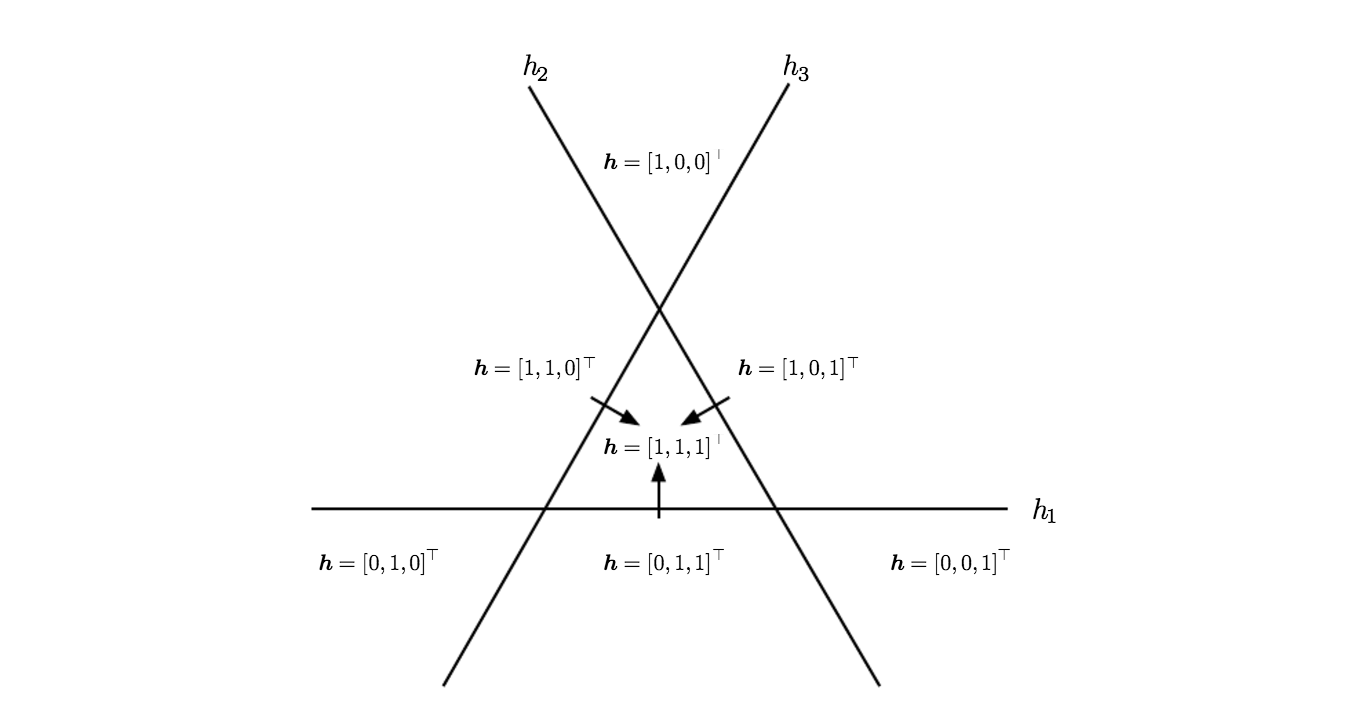
\includegraphics[width=13cm]{fig/chap15/15_7.png}
\caption{基于分布式表征的学习算法如何把空间分成各种区域的解释。在这个例子中,有三个二值特征 $h_1$, $h_2$ 和 $h_3$. 每一个特征是对所学习的线形变换的输出取阈值而得到。每一个特征把 $\mathbb{R}^2$ 分成了两个半平面。 $ h^+_i$ 表示 $h_i = 1$ 的输入点的集合, $h^-_i$ 表示 $h_i = 0$ 的输入点的集合。 在这个图示中,每条线代表了某个 $h_i$ 的决策边界,对应的箭头指向边界 $h^+_i$ 的一侧。 在这些半平面的每一个交界区域表征都有一个唯一的值。例如,在 $h^+_1 \cap h^+_2 \cap h^+_3$ 区域对应着表征值 $[1,1,1]^T$. 可以和图 \ref{fig:15_8} 中的非分布式表征对比一下。 在输入维为 d 的一般情况下,一个分布式表征用半空间,而不是半平面,把空间 $\mathbb{R}^d$分割开来。带有 $n$ 个特征的分布式表征要给 $O(n^d)$ 分配唯一的特征值,然而带有 $n$ 个样本的最近邻算法只需要给 $n$ 个区域分配特征值。相比于非分布式表征,分布式表征可以区分非常多的区域。需要记住的是,不是所有的 $h$ 值都是可行的(在这个例子中是没有 $h = 0$ 的),而且在分布式表征上的线形分类器不能给每一个周边区域都给予不同的类别,即使是一个 VC 维为 $O(\omega log \omega)$ 深度的线形阈值网络, 其中 $\omega$ 为权重的数量 (\textcolor{green}{Songtag, 1998}). 一个很强的表征层和一个弱的分类器层的结合可以是一个很强的正则器;一个分类“人”和“非人”的分类器没有必要区分“戴眼镜的女人”和“不戴眼镜的男人”。 这个容量的限制使得每一个分类器关注很少的 $h_i$, 并且使得 $\bf h$ 以一种线形分割的方式来学习去表达类别。}
\label{fig:15_7}
\end{figure}

\begin{figure}[h!]
\centering
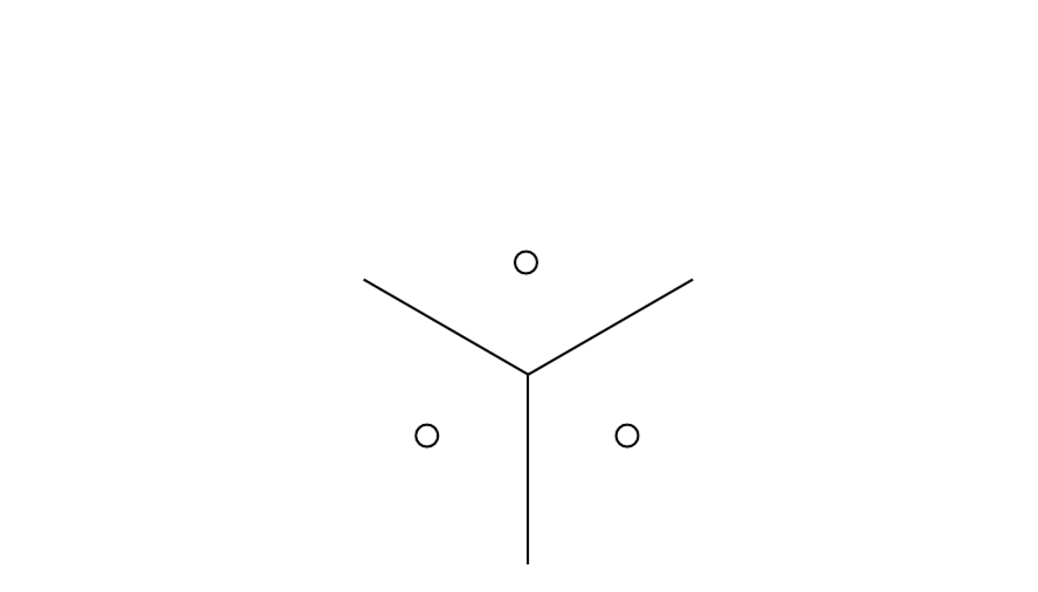
\includegraphics[width=13cm]{fig/chap15/15_8.png}
\caption{最近邻算法如何把输入空间分成不同区域的示例。最近邻算法是一个基于非分布式表征的学习算法的一个例子。不同的非分布式算法可能有不同的几何形式,但是它们都会把空间分成不同区域,每个区域都有一些独立的参数。非分布式的优势是,如果给充足的参数,它能在不用解决困难的优化问题情况下来拟合训练集合,因为它能很直接的对不同区域选定不同的输出值。它的缺点是这样的非分布式模型只能通过平滑先验来做局部概括,这使得它很难去学习凸点和凹点比样本数量多的复杂函数。参见图 \ref{fig:15_7}, 可以对比分布式表征。}
\label{fig:15_8}
\end{figure}

对一些非分布式的算法,输出有些不是恒定的,相反是附件区域的插值。 参数(或者样本)的数量和区域数量的关系是线形的。

一个重要的区别分布式表征和符号表征的相关概念是因为不同概念之间共同特征的普遍性。但做单纯的符号来看, “猫” 和 “狗” 这两个符号会离的比较远。 然而,如果一个东西可以用有意义的分布式表示和其它相联系,对于猫的很多事情都可以概括成狗的,或者相反。例如,我们的分布式表征可能包含比如“有毛发”或者“腿的数量”的条目,这些条目对"猫“和”狗“的嵌入表示有相同的值。正如 \ref{sec:12.4}章节,在对词的分布表示上的神经语言模型比在对词的 one-hot 表示上的模型概括的更好。分布式的表示可以引出一个很好的相似空间,在这个空间中,语义上相似的概念在距离上非常近,这个特点是符号表征所没有的。

使用分布式表征作为学习算法的一部分,什么时候和为什么有统计学上的优势?当明显复杂的结构能用很少的参数紧凑的表示时,分布式表征能有统计上的优势。一些典型的非分布式学习算法能有概括的效果,得益于平滑的假设,这个假设是说当 $u \approx v$,目标函数 f 可以学习到 $f(u) \approx f(v)$ 相似的特性。有很多方法可以形成这个假设,但是最后的结果是如果我们有一个样本 $(x, y)$ 并且 $f(x) \approx y$, 我们就可以选择一个估计器 $\hat{f}$, 它可以近似的满足这个约束,当移动到其临近输入 $x+\epsilon$ 时只需要改变尽可能小。这个假设是非常有用的,但是它会遭受到维数灾难。为了学习到目标函数,它能在许多区域增长和降低许多次\footnote{我们可能想要学习一个函数,它在许多区域都不同:在至少需要 2 个不同值去区分每个维度的 d-维空间中,我们可能想要 f 需要$O(2^d)$训练样本在区分$2^d$个不同的区域},我们可能需要大量的输入样本,至少和可区分的区域是一样大的。我们可以把每一个区域想象成一个类别或者符号,通过对每一个符号(或者区域)有不同的自由度,我们可以学习到任意的从符号到数值的解码器。然而,这个不能让我们对新的区域概括出新的符号。

如果我们幸运的话,除了平滑,在目标函数上可能有其它规则。比如, 即使在输入空间中物体的空间变换和平滑变换不对应,一个带有最大池化的卷积网络能识别物体,而不管它在图像中的位置。

让我们看分布式学习算法的一个特例,它能通过对输入的线形函数阈值化来提取二值特征。在这个表征中每一个二值特征都把空间$\mathbb{R}^d$分割成一对半空间,就像图 \ref{fig:15_7} 展示的那样。这些半空间之间的交叉空间的数量是对 n 成指数增长的,它决定了分布式表征学习器能区分多少区域。在 $\mathbb{R}^d$ 的 n 个超平面的组合能产生多少区域呢 ? 通过应用关于超平面的交叉区域( \textcolor{green}{Zaslavsky, 1975})的通用结果,  我们可以知道(\textcolor{green}{Pascanu et al, 2014b})二值特征表示能识别的区域数量是:
\begin{equation}
	\sum_{j=0}^d \binom{n}{j}= O(n^d)	
\label{equ:15.4}
\end{equation}
所以,我们可以看到它对于输入大小是指数的, 对隐含变量的数量是多项式的。


这给出了一个几何学的论据来解释分布式学习的概括能力: 如果有 $O(nd)$ 参数(在 $\mathbb{R}^d$ 中对 n 个线形阈值化特征),我们能在输入空间中区分 $O(n^d)$ 个区域。如果我们对所有数据没有任何假设,而是用一个符号代表一个区域的表征,并用对每一个符号用单独的参数来识别 $\mathbb{R}^d$ 中的对应区域,那么识别 $O(n^d)$ 区域需要 $O(n^d)$ 个样本。更通用的,对于分布式表征的论据可以扩展到其它的样本,这里我们对分布式表征的每一个属性不用线形,而是用非线形,可能还是连续的特征提取器。在这个例子中的论据是,如果一个有 k 个参数的参数变换能学习输入空间中的 r 个区域,这里 $k \ll r$,  并且如果这个表征对这个任务非常有用,相比较于我们需要 $O(r)$ 个样本来得到相同的特征和把输入空间变成 r 个区域的分割这样的非分布式的方式,我们用这个方式很大可能可以概括的更好。用更少的参数去表示网络意味着我们用更少的参数去拟合,所以需要更少的训练样本来概括。

基于分布式表征的模型能很好概括的更近一步的原因是尽管它能编码很多不同的区域,但它的容量是有限的。例如,带有线形阈值单元的神经网络的 VC 维是 $O(\omega log \omega)$, 其中 $\omega$ 是权重的数量(\textcolor{green}{Sontag, 1998})。有个局限是,当我们能把许多唯一的编码分配给表征空间时,我们不会用到所有的编码空间,我们也不能学习从表征空间 $\bf h$ 到输出 $\bf y$ 的带有线形分类器的任何函数。分布式表征结合线形分类器的使用展示了先验信念,被识别的类别是线形可分的,它是以被 $\bf h$ 所得的基本因果因子的函数的形式。我们希望去学习类别,比如所有包含绿色物体的图像集合,或是所有车的图像集合,但是不是需要非线形和 XOR 逻辑的类别。比如,我们把数据分割成所有红车和绿卡车的集合,以及绿车和红卡车的集合。


\begin{figure}[h]
\centering
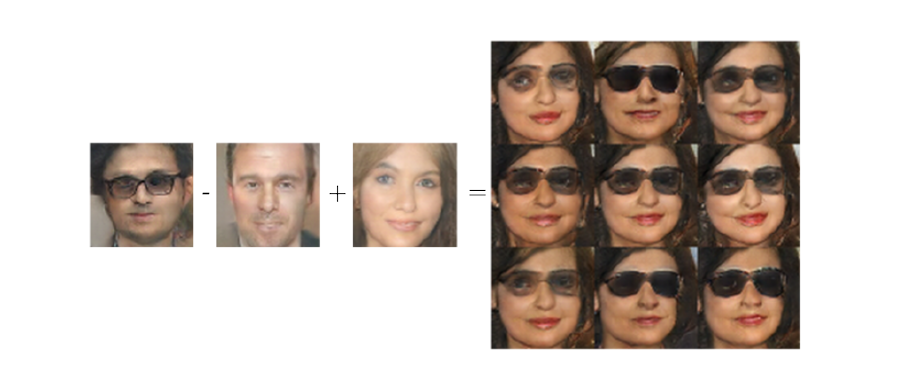
\includegraphics[width=13cm]{fig/chap15/15_9.png}
\caption{一个基于分布式表征的生成式模型,可以区分性别和戴不戴眼镜。如果我们先有一个戴眼镜的男人的表征,然后我们减去不戴眼镜的男人的向量表征,最后加上不戴眼镜的女人的向量表征,我们会得到戴眼镜的女人的表征。生成式模型把所有表征向量解码成对应的图像。 图像出自 \textcolor{green}{Radford et al. (2015)}}
\label{fig:15_9}
\end{figure}


目前讨论的想法都是抽象的,但是还需要实验来证实。 \textcolor{green}{Zhou et al.}( \textcolor{green}{2015}) 发现在 ImageNet 和  Place 数据集上根据人为赋予的标签训练出的深层卷积网络中的隐含单元所学的特征是可解释的。在实际中,并不是所有情况下,隐含单元都能学到带有语言学意义的特征,很有意思的是可以看到它们在接近视觉深层网络的顶层上出现。这些特征的共性是可以想象学习他们中的每一个而不用去看其它所有的配置。 \textcolor{green}{Rasford et.al (2015)} 展示生成模型可以学习人脸图片的表示,这个表示中每一个单独的方向都对应着变化的不同基本因子。图 \ref{fig:15_9} 说明了表征空间的一个方向对应着这个人是男是女,其它的一个方向是这个人是否带了眼镜。这些特征是自动被发现的,不是固定了先验。我们不需要把标签给隐藏单元分类器:对目标函数的梯度下降方法可以学习到有趣的语义特征,只要任务需要这些特征。我们可以学习到男和女的区别,或者戴与不戴眼镜的区别,这些都不用包含其它 n-1 个特征值的组合的例子来描述其它 n -1 个特征的配置。这种统计上可分离的形式可以使我们概括出人的特征的一种新的配置,可能它在训练中没有被看到。






















%%%%%%%%%%%%%%%%%%%%%%%%%%%%%%%
%%          15.5
%%%%%%%%%%%%%%%%%%%%%%%%%%%%%%%

\section{深度上带来的指数增益}
\label{sec;15.5}
在 \ref{sec:6.4.1} 节中我们看到多层感知机是通用逼近的,相比于浅层网络,一些函数是可以被小的深层网络所表示的。在模型大小上的减少可以导致统计效率上的提高。在这个章节中,我们会描述相似的结果是怎么适用到其它带有分布式隐含表示的模型中。

在 \ref{sec:15.4} 节中,我们看到生成式模型的一个例子,它能学习到人脸图片的可解释性的因素,包括人的性别和他们是否佩戴眼镜。能胜任这个任务的生成式模型式是基于深度神经网络。希望比如线形网络的浅层网络能学习到抽象可解释性因素和图像像素之间的复杂关系是不合理的。在这个和其它人工智能任务中,这些对应着有意义的输入的独立因素是比较高层级的,并且和输入是严重的非线形关系。我们需要争论的是我们需要深度分布式表征,高层次的特征(输入函数)或者因子(生成的原因)是由许多非线性组合得到的。

在许多配置下已经被证明了,除了通过分布式表征带来的提高,通过很多非线形的组合在计算和层次化的重用特征对统计效率有很大的提高。很多有一个隐含层的网络(e.g., 带有饱和非线形,布尔门,和/乘积,或者 RBF 单元)被证明是通用逼近的。如果有足够的隐含单元,一个通用逼近的模型簇可以在零容忍的程度上逼近非常多的函数(包括所有连续的函数)。 然而,需要的隐含单元的数量可能非常大。关于深层结构的表达能力的理论结果说明有有些函数簇可以被深度为 k 的结构有效的表示,但是对不深的结构(深度为 $2$ 或 $k-1$ )需要对输入大小呈指数级数量的隐含单元。

在 \ref{sec:6.4.1} 章节中, 我们看到确定的前向网络是函数通用逼近的。许多有一个隐含层的结构性的概率模型都是概率分布的通用逼近,包括有限玻尔兹曼机和深度置信网络( \textcolor{green}{Le Roux and Bengio, 2008, 2010; Montufar and Ay, 2011; Montufar, 2014; Krause et.al 2013})

在 \ref{sec:6.4.1} 章节中,我们看到充分深的前馈网络比浅网络有非常大的优势。对于其它模型(比如概率型模型)都有同样的结果。其中一个这样的概率模型是和积网络或 SPN ( \textcolor{green}{Poon and Domingos, 2011} ).  这些模型用多项式回路来计算在一些随机变量上的概率分布。\textcolor{green}{Delalleau and Bengio ( 2011 )} 展示了用最少深度的SPN,避免了大模型,来计算概率分布是存在的。随后,\textcolor{green}{Martens and Medabalimi ( 2014 )} 展示了每两个有限深度的 SPN 是有很大区别的,那些让 SPN 更容易处理的限制会限制他们的表达能力。

另一个有趣的发展方向是对类似卷积网络的深层回路这一类的表达能力的理论结果,它强调了深度回路的巨大优势,即使是浅层的回路去近似深度回路所学的函数 \textcolor{green}{(Cohen et al.2015)}. 对比一下可以看到,之前的理论工作都是针对浅层回路学习特定函数这样的例子。











%%%%%%%%%%%%%%%%%%%%%%%%%%%%%%%
%%          15.6
%%%%%%%%%%%%%%%%%%%%%%%%%%%%%%%

\section{提供发现基本原因的提示}
\label{sec:15.6}
为了结束这个章节,我们回到一个之前的问题上:是什么使一个表征比另一个好 ?在 \ref{sec:15.3} 章节中第一次介绍过,一个答案是一个理想的表征可以把生成数据的所有基本因素都找到,尤其是那些和我们的应用相关的因素。表征学习的大多数策略是基于给学习算法提供提示来帮助他们找到这些基本因素。这些提示能帮助学习算法区别这些基本因素。监督学习提供了非常强的提示:对每一个 $\bf x$ 都有标签 $\bf y$, 它至少设定了一个变化方向上的值。更一般的,为了利用大量无标签的数据,表征学习要非直接的利用提示来得到这些基本因素。这些以隐式的先验形式的提示被引入来引导学习算法。没有免费午餐定理的结果说明正则策略对得到好的概括很有必要。虽然找到通用的非常好的正则策略是不可能的,但是深度学习的一个目标是找到一些通用的公平的正则策略,它们能适用到很多人和动物能解决的人工智能任务上。

我们提供了这样的通用的正则策略的一个列表。这个列表显然是不完全的,但它给出了具体的例子,它们能帮助发现对应基本因子的特征。这个列表在 \textcolor{green}{Bengio et.al (2013d)} 的 3.1 章节中被介绍过,在这里我们拓展一下。

\begin{itemize}
	\item 平滑性: 这个假设是对单元 $\bf d$ 和小的 $\epsilon$ 有 $f(\bf x+\epsilon d)\approx f(x)$ 这个假设可以让学习算法在输入空间中从训练样本概括到临近的点。许多机器学习算法都利用这个想法,但是还是不足以克服维数灾难。

	\item 线形性: 许多机器学习算法都假设变量之间的关系是线形的。这个可以使算法得到的预测离观测数据非常远,但是有时候会得到非常极端的预测。许多不用平衡假设的简单的机器学习算法使用了线形的假设。这些是不同的假设——针对高纬度空间的含有大量参数的线形函数可能不是非常平滑。可以参见 \textcolor{green}{Goodfellow et al. (2014b)} 得到关于线形假设局限性的更多讨论。

	\item 多解释性因子:许多表征学习算法都因为一个假设,数据的生成是基于很多基本都可解释因子,大部分任务都可因它们而简单地被解决。\ref{sec:15.3} 章节描述了这个观点是如何通过表征学习来启发半监督学习的。学习 p(x) 的结构需要学习对 p(y|x)建模有用的一些相同的特征,因为这些特征都对应着相同的基本可解释因子。\ref{sec:15.4} 章节这个观点是如何启发了分布式表征的使用,它在表征空间中每一个单独的方向都对应着变化的一处因子。

	\item 因果因子:模型是以把所学表征 $\bf h$ 所描述的变化因子当做所观测数据 $\bf x$ 的来源这样的方式来构建的,而不是相反的过程。正如 15.3 章节讨论的,这个是半监督学习的优势,并且使得当对基本原因的分布变化时或者当我们对一个新的任务使用这个模型时,所学的模型更加鲁棒。

	\item 深度,或者可解释因子的层级结构: 高层级,抽象的概念被定义成形成层级的简单概念。从另一个点来说,深度结构的使用表达了我们的任务应该被多步程序所实现这样的观点, 每一步都根据前一步的输出。

	\item 任务之间共享的因子: 在有很多任务的情况下,对应着共享相同输入 $x$,或者每一个任务都对应着一个子集,或者对应着一个全局输入 $x$ 的函数 $f^{(i)}(x)$ 的不同的 $y_i$, 每一个 $y_i$ 都对应着相关因子 $h$ 的不同子集。因为这些子集的重合,通过共用的中间表征 $P(h|x)$ 来学习所有的 $P(y_i|x)$ 允许在任务之间共享统计的优势。 

	\item 流形: 概率质量集中在的区域是局部连接,它们只占了很小的体积。在连续的情况下,这些区域都被低维的流形来近似,这些流形比数据的原始空间有更少的维度。许多机器学习算法对这些流形都比较敏感 \textcolor{green}{Goodfellow et al, 2014b}. 一些机器学习算法,尤其是自编码器,尝试显示的去学习流形的结构。

	\item 自然聚类:许多机器学习算法假设在输入空间中每一个相连的流形都可能分配到一个单独的类别中。数据可能会在不相通的流形上,但是类别是保持不变的。这个假设引起了很多学习算法,包括切线传播,双后项传播,流行切线分类器和对抗训练。

	\item 时间和空间的相关性:慢特征分析和相关的算法有一个假设,大多数重要的可解释性的因子变换地都比较慢,或者至少它能较为简单的预测基本的可解释性因子,而不是预测原始的观测值,比如像素值。关于这个方法更多的描述可以参见 \ref{sec:13.3} 章节。

	\item 稀疏性:大多数特征不应该描述大多数输入——没有必要去用检测大象主干的特征去表示带有猫的图。 所以,“有”和“没有”这样的特征不应该在大多数情况下出现是比较合理的。

	\item 因子依赖的简单性:在好的高层级的表征时,相关的因子之间是简单依赖的。最简单的可能是边际独立,$P(h) = \prod_{i} P(h_i)$,  但是线形依赖或者浅层的自编码器所展示的那些都是合理的假设。这些在很多物理规律中都可以看到,当把线形预测器和因子先验放在所学表征的顶端时,它是假设成立的。
\end{itemize}

表征学习的概念和其它深度学习的形式都有关联。前馈和循环网络,自编码器以及深度概率模型都能学到和发现表征。学到尽可能好的表征仍然是有趣的研究方向。
































